
%\begin{figure*}[ht]
%	\raggedleft
%	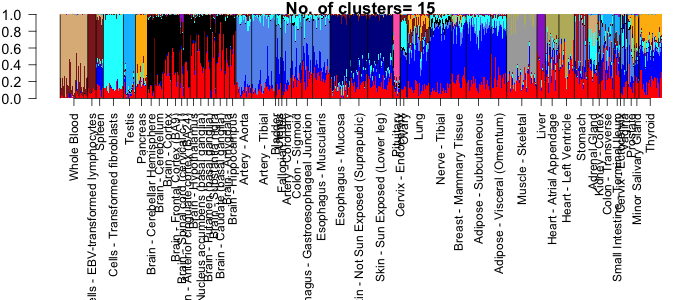
\includegraphics[height=3in, width=6.5in]{../plots/whole_tissue_structure_15.png}
%        \caption{Structure plot of the admixture proportions (with 15 topics/clusters) for all the tissue samples in GTEX Version 4 data based on $5000$ genes with the highest mean expression. Some of the tissues form very distinct clusters, for instance Whole Blood, Pancreas, Skin, Arteries etc while there is a lot of similarity in cluster patterns between Muscle Skeletal and Heart Left Ventricle, or among the different sub-tissues of the Brain.}
%\end{figure*}

\begin{sidewaysfigure*}[ht]
\raggedleft
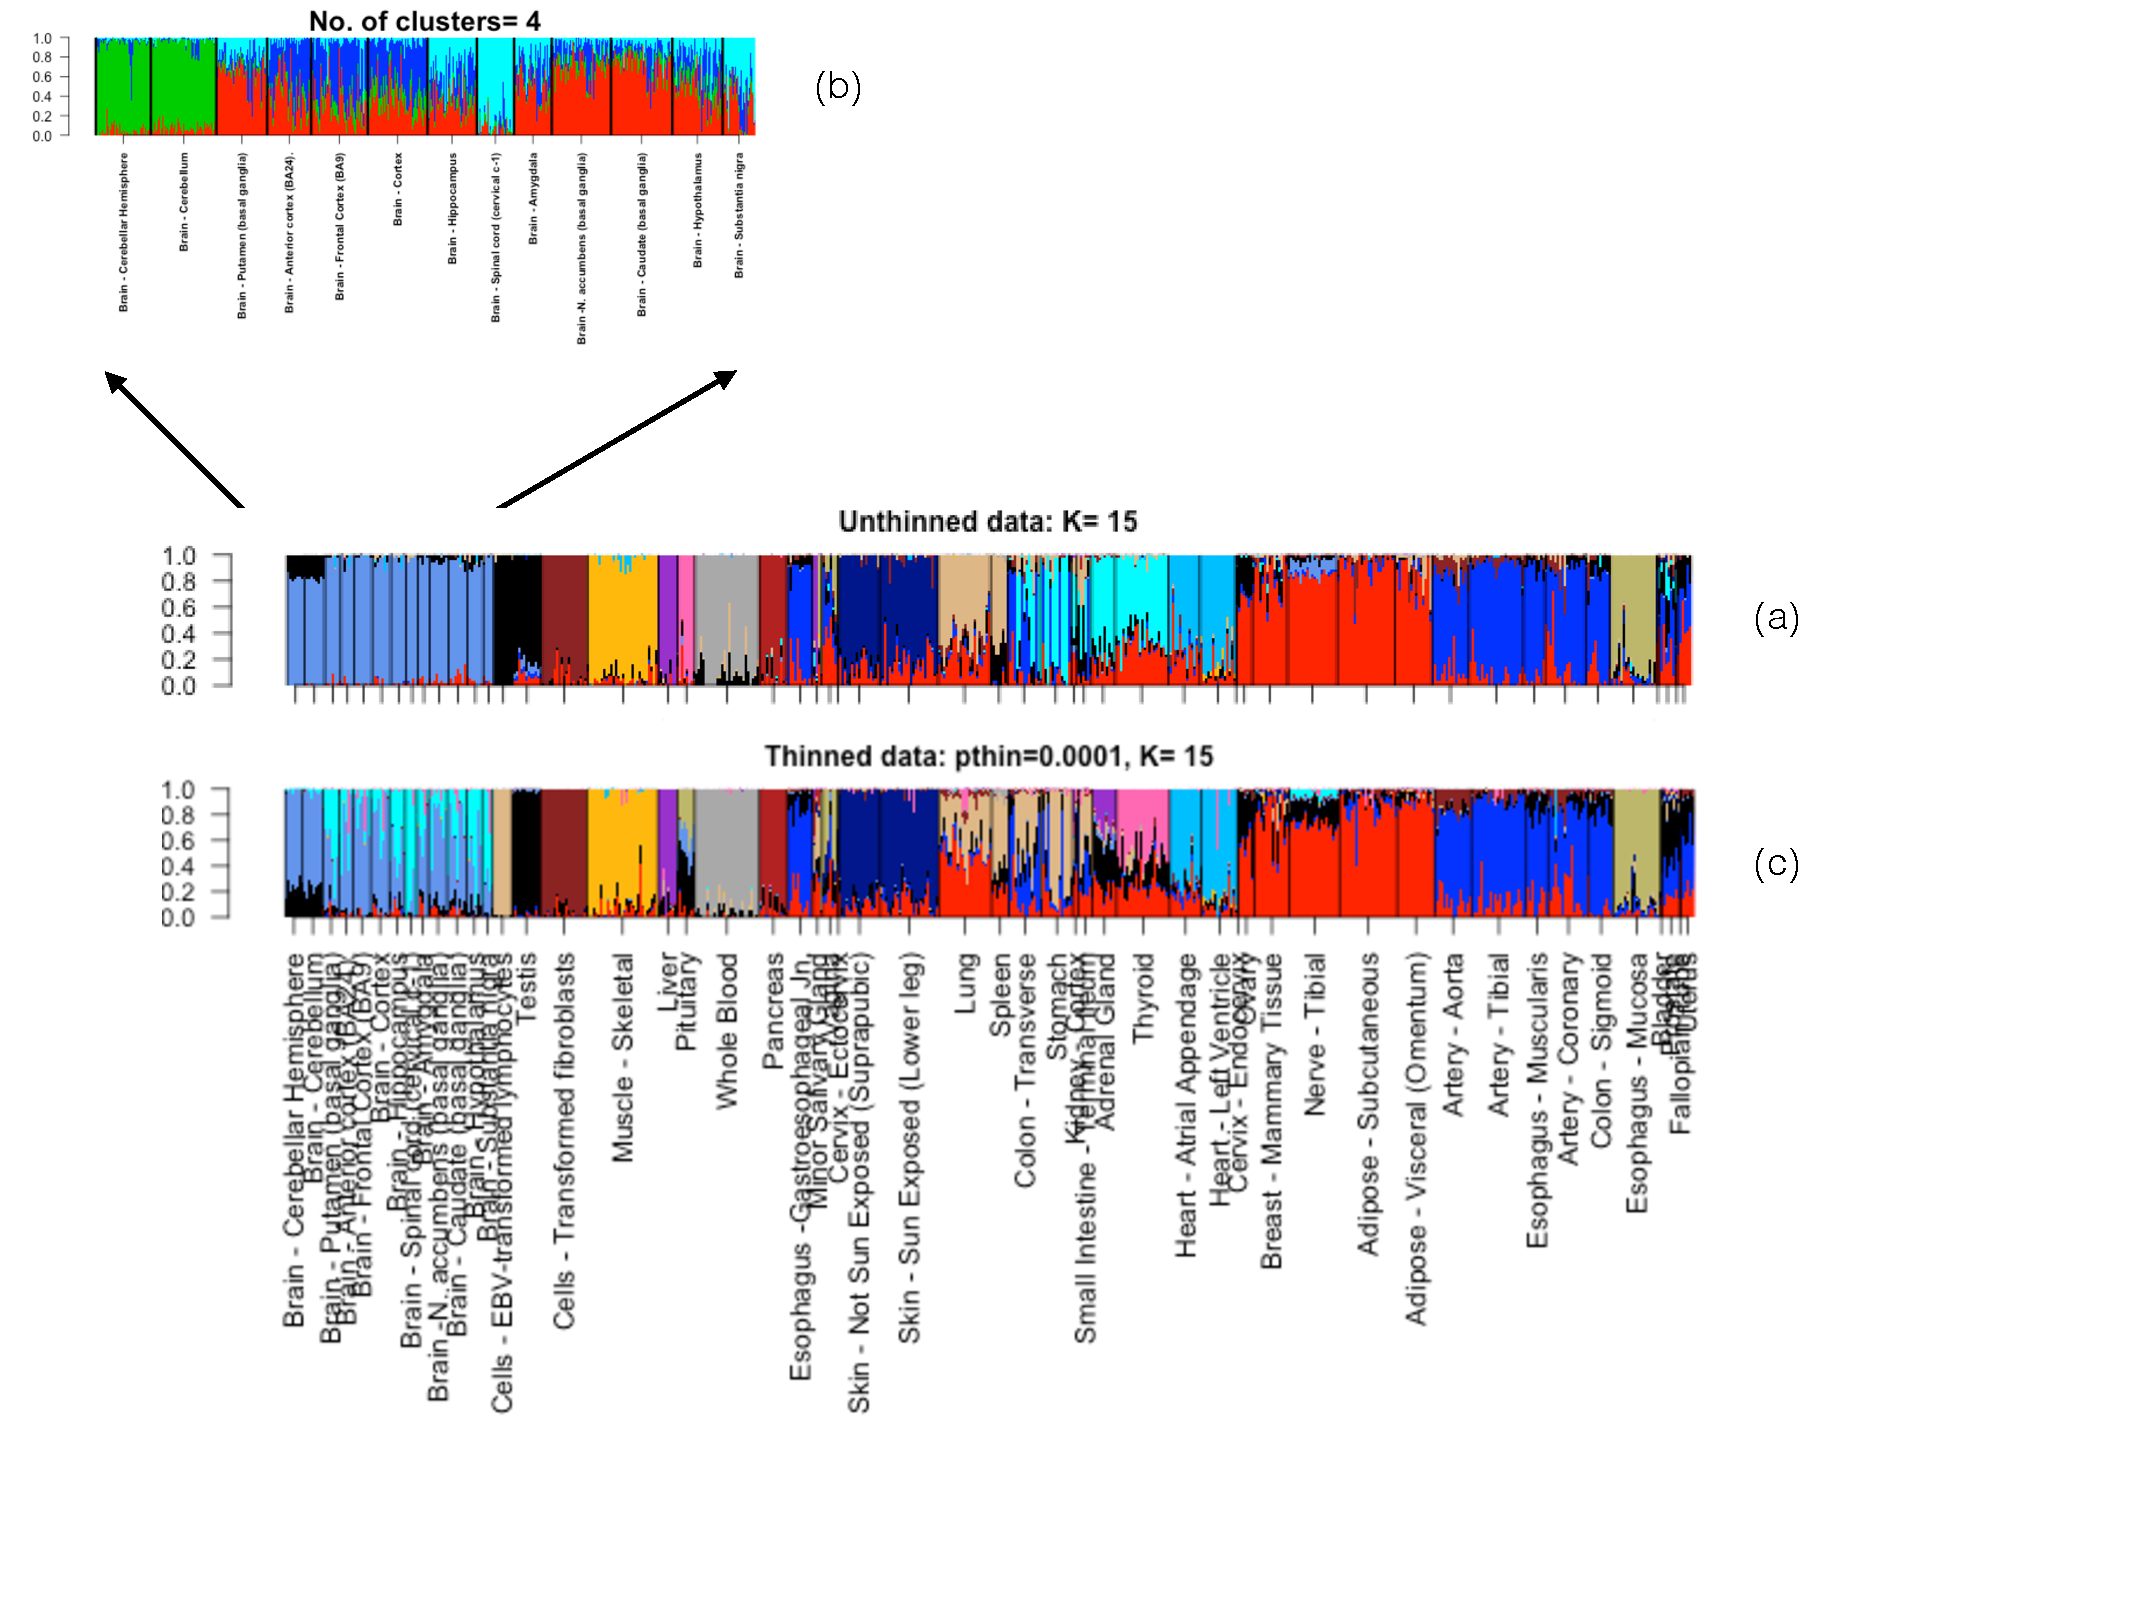
\includegraphics[height=5in, width=6.5in]{../plots/gtex-figures/fig1.pdf}
 \caption{ \textbf{(a)}: Structure plot of estimated cluster membership proportions for $K=15$ clusters fit to $8555$ tissue samples from $53$ tissues in GTEX data.  Each vertical bar shows the cluster membership proportions for a single sample, ordered so that samples from the same tissue are adjacent to one another. \textbf{(b)}: Structure plot of estimated cluster membership proportions for $K=4$ clusters fit to only the brain tissue samples from GTEX. This analysis highlights finer-scale structure among the brain samples that is absent from (a).  \textbf{(c)}: As in a), but with data thinned so that the coverage is closer to a typical single cell RNA-seq data ($p_{thin}=0.0001$).  The clustering patterns are largely similar to a), but slightly noisier.}
\label{fig:fig1}
\end{sidewaysfigure*}
%
%\begin{figure*}[ht]
%\centering
%  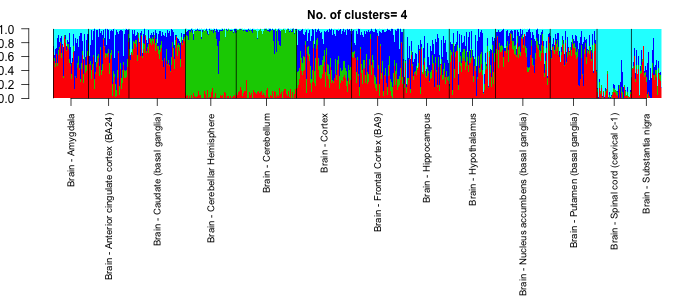
\includegraphics[height=3in, width=4.5in]{../plots/GTEX_V6_brain_thin_0.png}
%    \caption{Structure plot of the admixture proportions (with 4 clusters) for the brain tissue samples drawn from GTEX Version 4 data. Quite clearly, brain cerebellum and cerebellar hemisphere seem to be dominated by the blue cluster while the Spinal cord and Substantia nigra by the cyan cluster. Prior marker based approaches have verified that $> 80 \%$ of cells in brain cerebellum correspond to neurons \cite{Houzel2005}. So, the blue cluster seems to be driven by the neuron cell type. This fact is further attested by the gene annotations of the top genes driving the blue cluster (Supplementary Table 1).}
%\label{fig:fig2}
%\end{figure*}
%
% \begin{figure*}[ht]
%        \centering
%        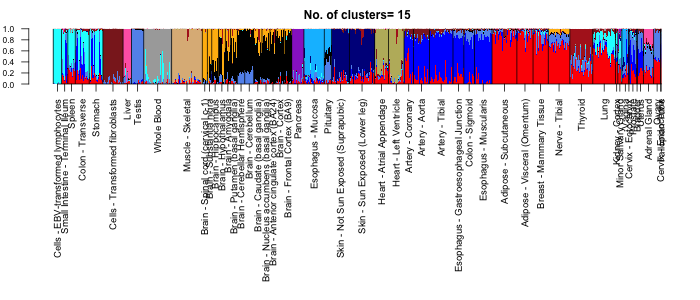
\includegraphics[height=2.7in]{../plots/GTEX_V6_thin_2.png}
%    \caption{Structure plot of all tissue samples in GTEx V6 data thinned data with $p_{thin}=0.0001$ for $K=15$. The thinning parameter has been chosen so that the GTEx RNA-seq data can be interpreted at the same scale as a scRNA-seq data.  The clustering patterns are more noisy compared to the non-thinned data in Fig \ref{fig:fig1}, but overall, the similarity patterns across the tissues are retained. For instance, the brain tissues and the arteries still seem to be clustering together.}
% \label{fig:fig4}
%    \end{figure*}


  \begin{figure*}[ht]
    \centering
    \begin{subfigure}[t]{0.5\textwidth}
        \centering
        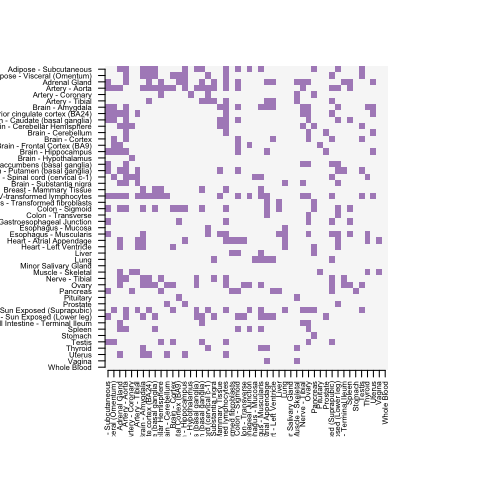
\includegraphics[height=2.5in]{../plots/hierarchy_F_thin_0_1.png}
        \caption{hierarchy thin 0.1}
    \end{subfigure}%
    ~ 
    \begin{subfigure}[t]{0.5\textwidth}
        \centering
        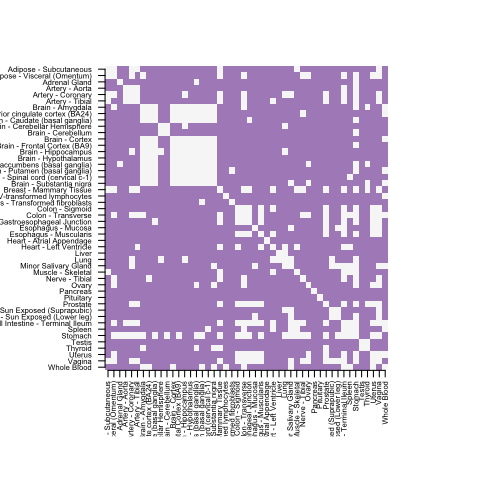
\includegraphics[height=2.5in]{../plots/admixture_F_thin_0_1.png}
        \caption{admixture thin 0.1}
    \end{subfigure} \\
\caption{A comparison of ``accuracy" of hierarchical vs model-based clustering. For each pair of tissues from the GTEX data we assessed whether or not each clustering method (with $K=2$ clusters) separated the samples according to their actual tissue of origin, with successful separation indicated by a filled square. Some pairs of tissues (e.g. pairs of brain tissues) are more difficult to distinguish than others. Overall the model-based clustering is successful in xx comparisons and the hierarchical clustering in yy comparisons.}
\label{fig:fig2}
\end{figure*}


    
    
%     \begin{figure*}[ht]
%    \raggedright
%     \begin{subfigure}[t]{0.25\textwidth}
%        \raggedleft
%        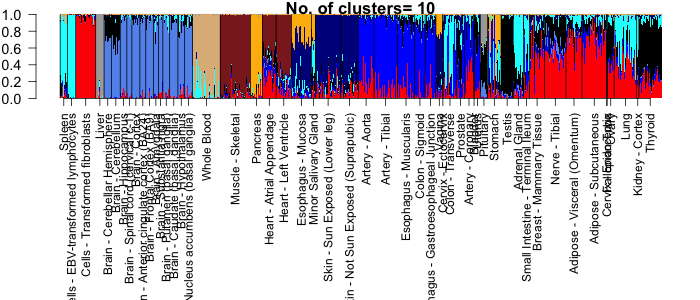
\includegraphics[height=2.5in]{../plots/multiple_thinned_1.png}
%        \caption{Run 1}
%    \end{subfigure}    \\
%    \begin{subfigure}[t]{0.25\textwidth}
%        \raggedleft
%        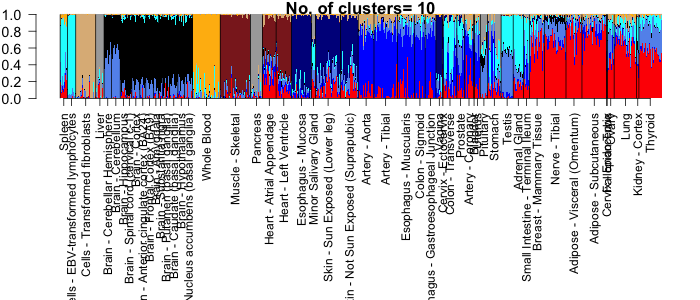
\includegraphics[height=2.5in]{../plots/multiple_thinned_2.png}
%        \caption{Run 2}
%    \end{subfigure}   \\
%    \begin{subfigure}[t]{0.25\textwidth}
%        \raggedleft
%        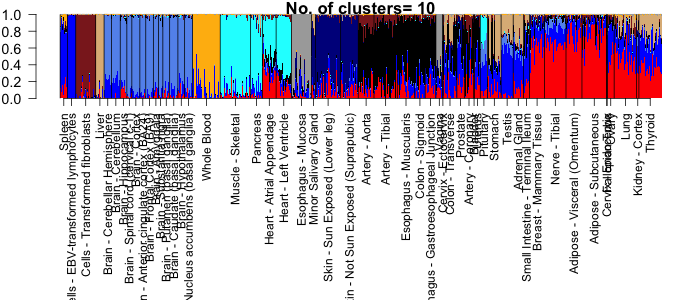
\includegraphics[height=2.5in]{../plots/multiple_thinned_4.png}
%        \caption{Run 3}
%    \end{subfigure} 
%    \caption{Structure plot of all tissue samples in 3 runs of the GTEx version 4 data for for K=10 for the thinning parameter $p_{thin}=0.01$. For the 3 runs, the datasets are randomly generated from the actual counts data using $p_{thin}=0.01$, so the datasets are different across the 3 runs. However, it seems the results are pretty robust.}
%    \end{figure*}
%
    
%    \begin{figure*}[ht]
%    \centering
%    \begin{subfigure}[t]{0.5\textwidth}
%        \centering
%        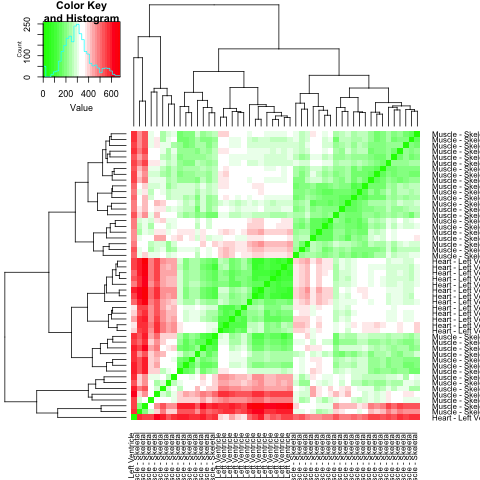
\includegraphics[height=2.5in]{../plots/heart_muscle_hierarchical_heatmap_complete.png}
%        \caption{counts- complete linkage}
%    \end{subfigure}%
%    ~ 
%    \begin{subfigure}[t]{0.5\textwidth}
%        \centering
%        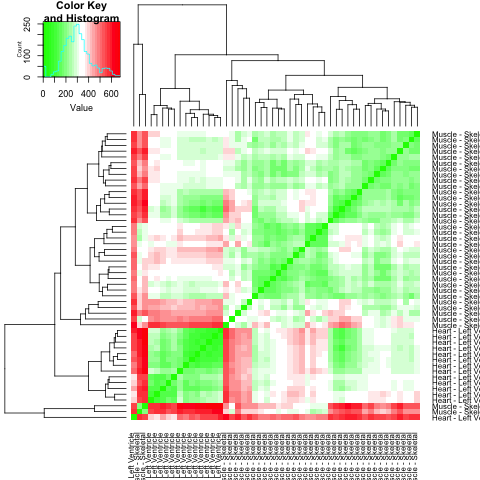
\includegraphics[height=2.5in]{../plots/heart_muscle_hierarchical_heatmap_average.png}
%        \caption{counts- average linkage}
%    \end{subfigure} \\
%    
%     \begin{subfigure}[t]{0.5\textwidth}
%        \centering
%        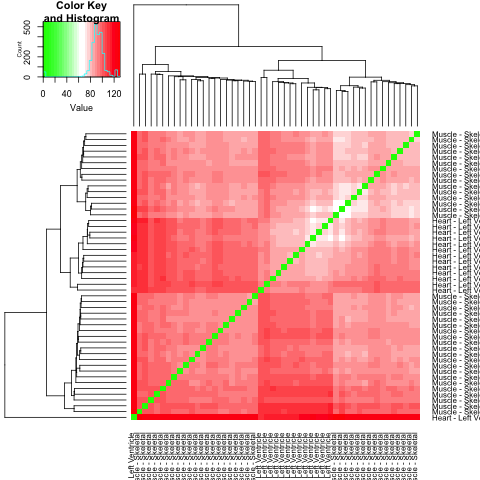
\includegraphics[height=2.5in]{../plots/heart_muscle_hierarchical_heatmap_cpm_complete.png}
%        \caption{cpm- complete linkage}
%    \end{subfigure}%
%    ~
%    \begin{subfigure}[t]{0.5\textwidth}
%        \centering
%        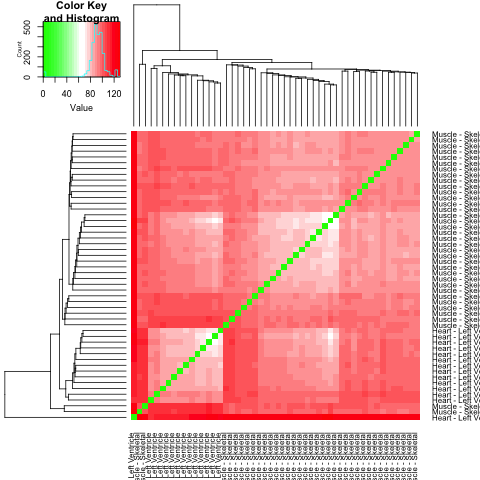
\includegraphics[height=2.5in]{../plots/heart_muscle_hierarchical_heatmap_cpm_average.png}
%        \caption{cpm- average linkage}
%    \end{subfigure}\\
%    
%     \begin{subfigure}[t]{0.5\textwidth}
%        \centering
%        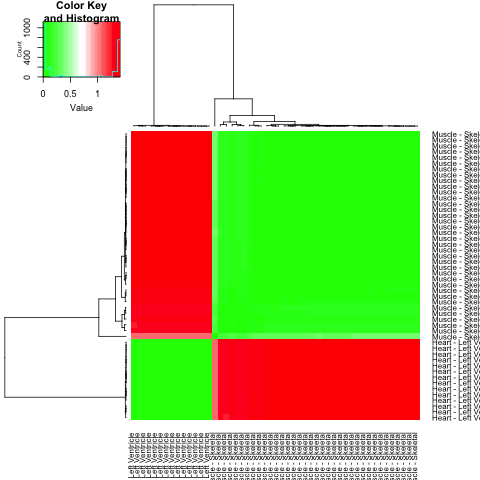
\includegraphics[height=2.5in]{../plots/heart_muscle_admix_heatmap_complete.png}
%        \caption{admix prop- complete linkage}
%    \end{subfigure}%
%    ~
%    \begin{subfigure}[t]{0.5\textwidth}
%        \centering
%        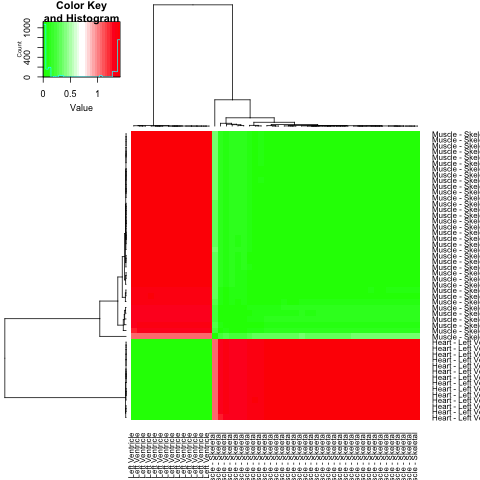
\includegraphics[height=2.5in]{../plots/heart_muscle_admix_heatmap_average.png}
%        \caption{admix prop- average linkage}
%    \end{subfigure}\\
%
%    \caption{Comparison of heatmap of the counts data (\textit{top panel}), the cpm normalized data (\textit{middle panel}) and the admixture proportions data (\textit{bottom panel}) on  a randomly drawn 50 samples from the pool of Muscle-Skeletal and Heart-Left Ventricle samples in GTEx Version 4 RNA-seq thinned counts data with the thinning parameter $p_{thin}=0.001$. The distance method used euclidean and the linkage used was average linkage. Color scale provided in the figure. It seems that for admixture model heatmap, all the Muscle-skeletal and Heart Left-Ventricle samples cluster separately, while for the hierarchical model heatmap, they are mixed with each other. This suggests Admixture is better equipped at picking tissue separation than hierarchical clustering.}
%\end{figure*}
%


%  \begin{figure*}[ht]
%    \centering
%    \begin{subfigure}[t]{0.5\textwidth}
%        \centering
%        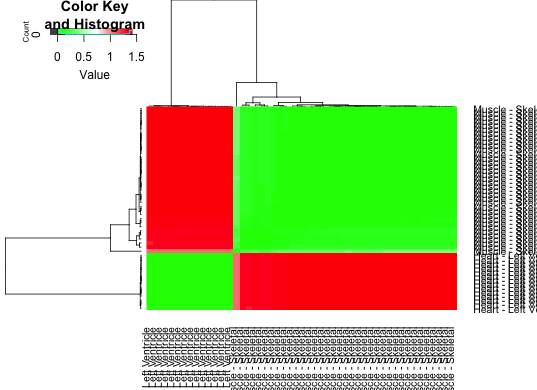
\includegraphics[height=2.5in]{../plots/hierarchical_admix_2.png}
%        \caption{k=2}
%    \end{subfigure}%
%    ~ 
%    \begin{subfigure}[t]{0.5\textwidth}
%        \centering
%        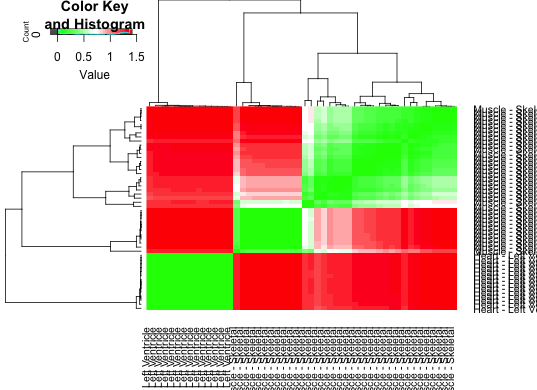
\includegraphics[height=2.5in]{../plots/hierarchical_admix_3.png}
%        \caption{k=3}
%    \end{subfigure} \\
%    
%     \begin{subfigure}[t]{0.5\textwidth}
%        \centering
%        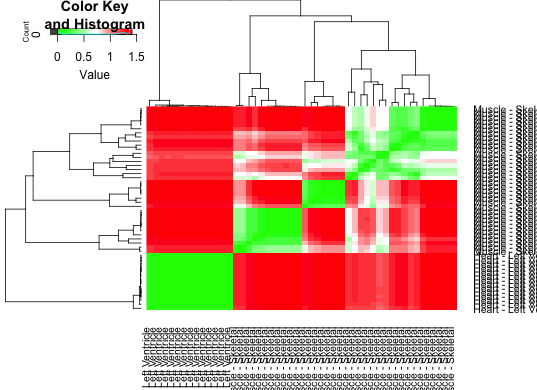
\includegraphics[height=2.5in]{../plots/hierarchical_admix_4.png}
%        \caption{k=4}
%    \end{subfigure}%
%    ~
%    \begin{subfigure}[t]{0.5\textwidth}
%        \centering
%        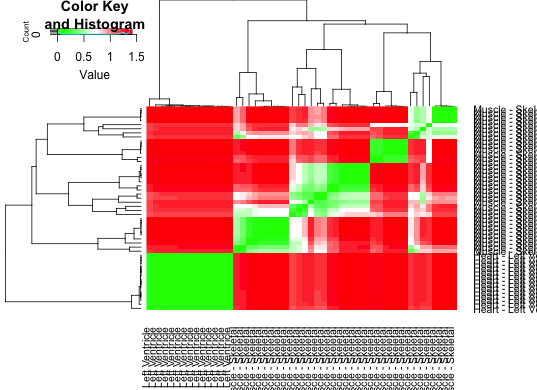
\includegraphics[height=2.5in]{../plots/hierarchical_admix_5.png}
%        \caption{k=5}
%    \end{subfigure}\\
%
% \caption{The heatmap of the admixture topic proportion matrix (low dimensional compared to the original counts data) under four different choices of clusters or topics namely $2,3,4$ and $5$. Here we assume complete linkage and the distance is taken to be Euclidean distance.}
%\end{figure*}

% \begin{figure*}[ht]
%    \centering
%    \begin{subfigure}[t]{0.5\textwidth}
%        \centering
%        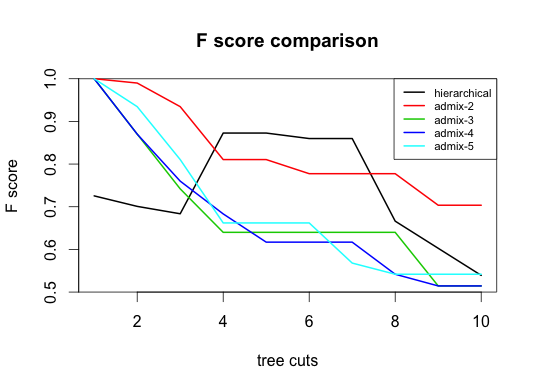
\includegraphics[height=2.5in]{../plots/Fscore_compare_average.png}
%        \caption{average linkage}
%    \end{subfigure}%
%    ~ 
%    \begin{subfigure}[t]{0.5\textwidth}
%        \centering
%        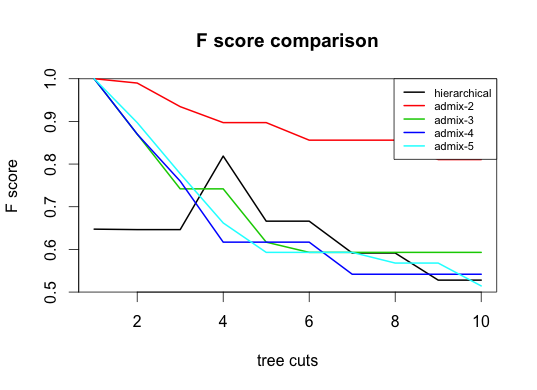
\includegraphics[height=2.5in]{../plots/Fscore_compare_complete.png}
%        \caption{complete linkage}
%    \end{subfigure} 
% \caption{The comparison of the F score of quality assessment between the hierarchical clustering on the actual counts data and the admixture model topic proportion matrix for number of topics $2$, $3$, $4$ and $5$. Higher values of $F$ imply better correspondence of the cluster labels with the pre-assigned class labels - in this case there being 2 classes, namely Muscle Skeletal and Heart Left Ventricle. The F scores are compared for both average and complete linkages.}
%\end{figure*}




%%\begin{figure*}[ht]
%    \centering
%    \begin{subfigure}[t]{0.5\textwidth}
%        \centering
%        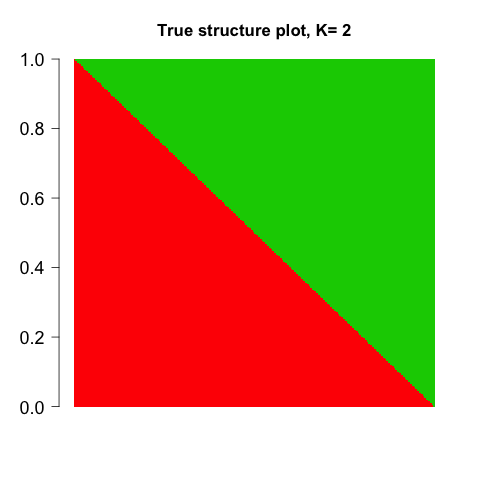
\includegraphics[height=3in]{../plots/true_structure_setup_1.png}
%        \caption{Set up 1 (true structure)}
%    \end{subfigure}%
%    ~ 
%    \begin{subfigure}[t]{0.5\textwidth}
%        \centering
%        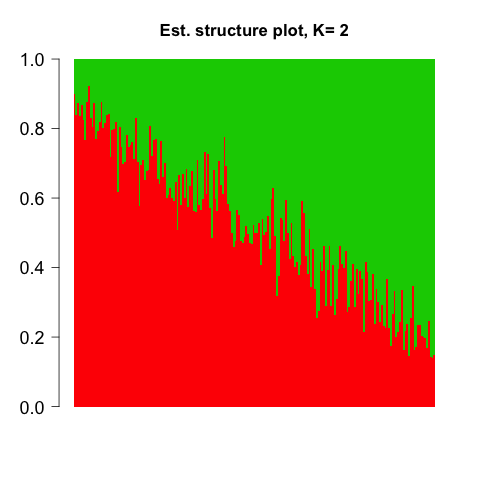
\includegraphics[height=3in]{../plots/est_structure_setup_1.png}
%        \caption{Set up 1 (est. structure)}
%    \end{subfigure}   \\
%    
%    \begin{subfigure}[t]{0.5\textwidth}
%        \centering
%        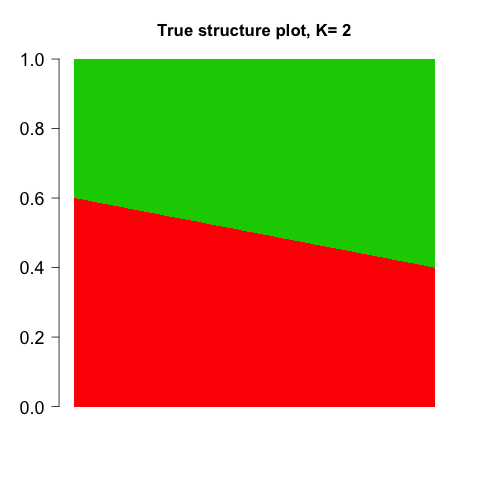
\includegraphics[height=3in]{../plots/true_structure_setup_2.png}
%        \caption{Set up 2 (true structure)}
%    \end{subfigure}%
%    ~ 
%    \begin{subfigure}[t]{0.5\textwidth}
%        \centering
%        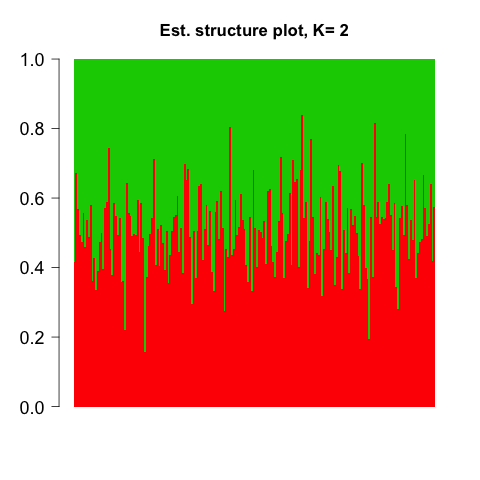
\includegraphics[height=3in]{../plots/est_structure_setup_2.png}
%        \caption{Set up 2 (est. structure)}
%    \end{subfigure} 
%    \caption{A case study to check for the performance of the admixture model under two set ups, one where the true admixture proportions vary a lot from 0 to 1 across samples for the two clusters and the other where the true admixture proportions vary mildly around $0.5$ (from $0.4$ to $0.6$) for the two clusters. It is found that the admixture model is able to distinguish the clusters better in the first set up compared to the second. Even from gene annotations point of view, it is found that the admixture model is able to extract the truly significantly enriched genes for the clusters in the first set up but fails to do so in the second set up.}
% \end{figure*}
% %
 
% \begin{figure*}[ht]
%    \centering
%    \begin{subfigure}[t]{0.5\textwidth}
%        \centering
%        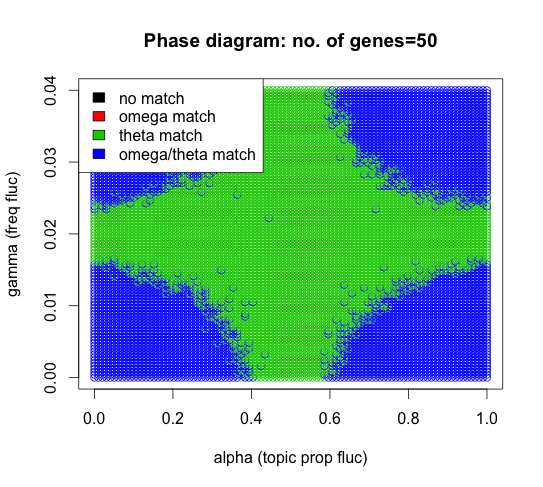
\includegraphics[height=3in]{../plots/phase_plot_50.png}
%        \caption{G=50}
%    \end{subfigure}%
%  ~ 
%    \begin{subfigure}[t]{0.5\textwidth}
%        \centering
%        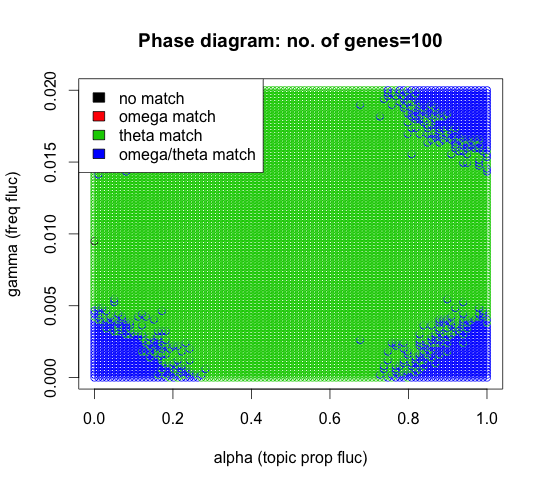
\includegraphics[height=3in]{../plots/phase_plot_100.png}
%        \caption{G=100}
%    \end{subfigure}   
%      ~ 
%    \begin{subfigure}[t]{0.5\textwidth}
%        \centering
%        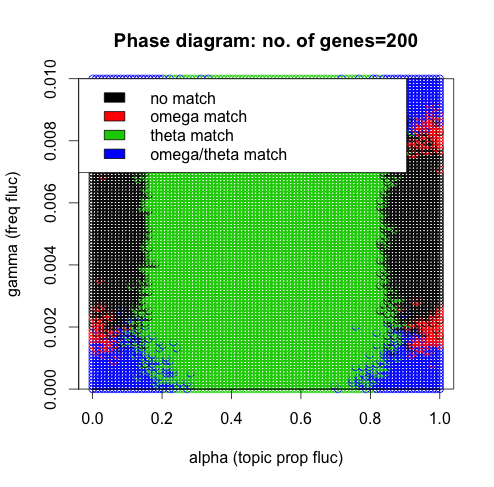
\includegraphics[height=3in]{../plots/phase_plot_200.png}
%        \caption{G=200}
%    \end{subfigure}   
%    \caption{Phase diagram analysis for number of samples $N=200$ and three choices of $G$, $50$, $100$ and $200$. Note that as $G$ increases, the gene expression signal and the distance between the relative gene expression between the two clusters decreases. As a result, the performance of the admixture model deteriorates. Also, for a broad part of the phase space, though the admixture model does not manage to determine the admixture proportions well enough (\textit{omega match} does not hold) but it is able to extract the actually important genes driving the clusters (\textit{theta match} holds).}
%    \end{figure*}
%    
 
% \begin{figure*}[ht]
%    \centering
%    \begin{subfigure}[t]{0.5\textwidth}
%        \centering
%        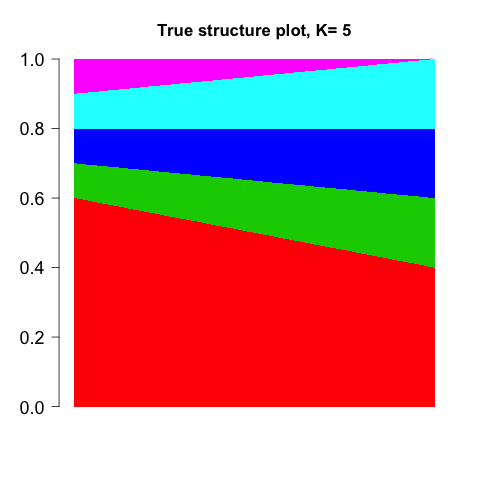
\includegraphics[height=3in]{../plots/true_structure_setup_3.png}
%        \caption{Set up 3 (true structure)}
%    \end{subfigure}%
%    ~ 
%    \begin{subfigure}[t]{0.5\textwidth}
%        \centering
%        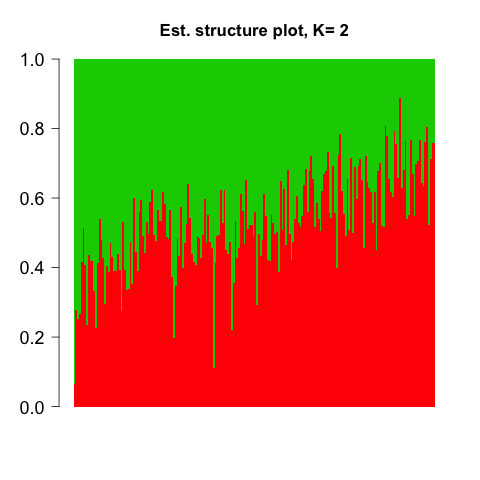
\includegraphics[height=3in]{../plots/est_structure_setup_3.png}
%        \caption{Set up 3 (est. structure)}
%    \end{subfigure}
%    \caption{The true structure plot for a simulation set up with $N=1000$ samples nd $G=500$ genes with $K=5$ clusters where the admixture proportions are given in (a). Counts data were generated under this true simulation set up. Then admixture model was fitted for $K=2$ and the estimated Structure plot from the model fit is shown in (b).}
%\end{figure*}

%\clearpage
%
%\begin{figure*}[ht]
%    \centering
%    \begin{subfigure}[t]{0.5\textwidth}
%        \centering
%        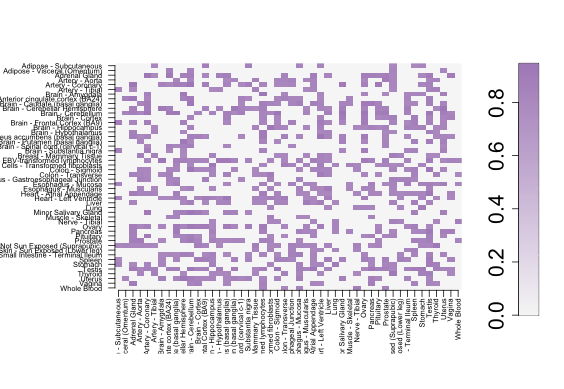
\includegraphics[height=2.5in,width=2.5in]{../plots/hierarchy_F_thin_clus_5_0_1.png}
%        \caption{hierarchy thin 0.1}
%    \end{subfigure}%
%    ~ 
%    \begin{subfigure}[t]{0.5\textwidth}
%        \centering
%        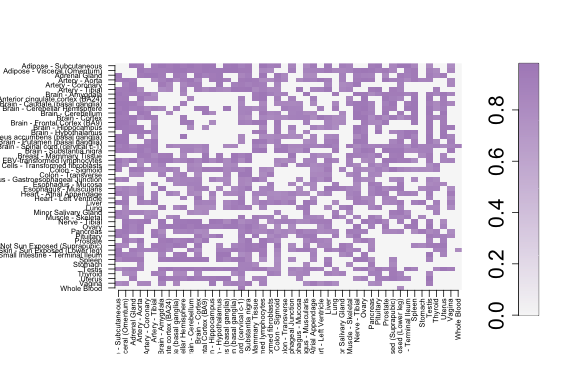
\includegraphics[height=2.5in,width=2.5in]{../plots/admixture_F_thin_clus_5_0_1.png}
%        \caption{admixture thin 0.1}
%    \end{subfigure} \\
%    
%     \begin{subfigure}[t]{0.5\textwidth}
%        \centering
%        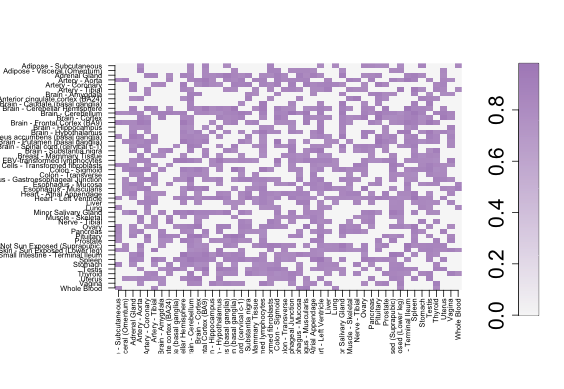
\includegraphics[height=2.5in,width=2.5in]{../plots/hierarchy_F_thin_clus_5_0_01.png}
%        \caption{hierarchy thin 0.01}
%    \end{subfigure}%
%    ~
%    \begin{subfigure}[t]{0.5\textwidth}
%        \centering
%        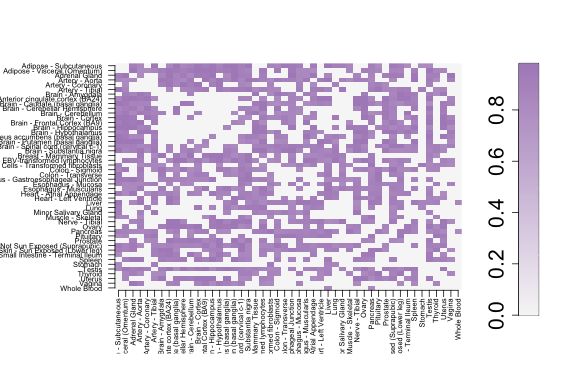
\includegraphics[height=2.5in,width=2.5in]{../plots/admixture_F_thin_clus_5_0_01.png}
%        \caption{admixture thin 0.01}
%    \end{subfigure}\\
%    
%     \begin{subfigure}[t]{0.5\textwidth}
%        \centering
%        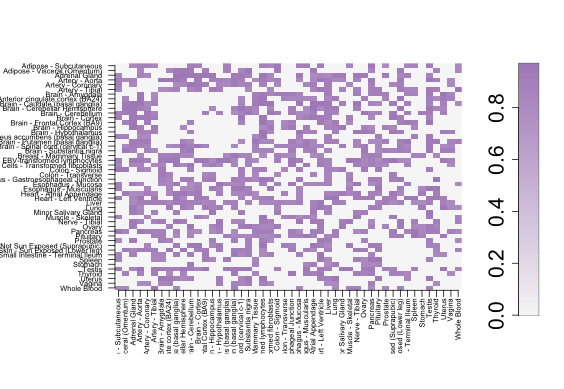
\includegraphics[height=2.5in,width=2.5in]{../plots/hierarchy_F_thin_clus_5_0_001.png}
%        \caption{hierarchy 0.001}
%    \end{subfigure}%
%    ~
%    \begin{subfigure}[t]{0.5\textwidth}
%        \centering
%        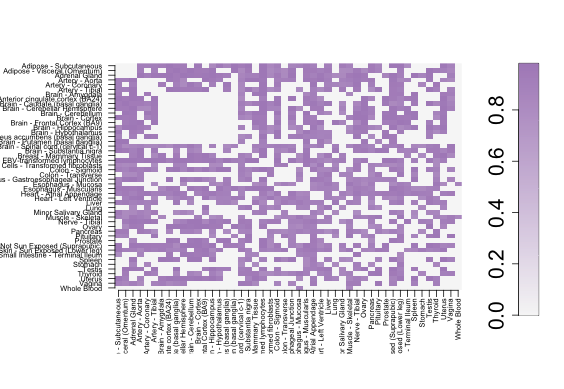
\includegraphics[height=2.5in,width=2.5in]{../plots/admixture_F_thin_clus_5_0_001.png}
%        \caption{admixture thin 0.001}
%    \end{subfigure}\\
% \caption{F score comparison of hierarchical clustering cut at 2 clusters on the actual counts data and on admixture proportions matrix  with 5 topics, where the F score is thresholded at $0.8$. In terms of F score, the performance of the admixture model in separating out the two clusters is much better than the hierarchical model. Also it seems that as we increase thinning, the performance does indeed deteriorate, as is intuitive. However, the relative efficiency of admixture over hierarchical clustering is maintained at all levels of thinning.}
%\end{figure*}
%
%

% \begin{figure*}[ht]
%    \raggedright
%     \begin{subfigure}[t]{0.3\textwidth}
%        \raggedleft
%        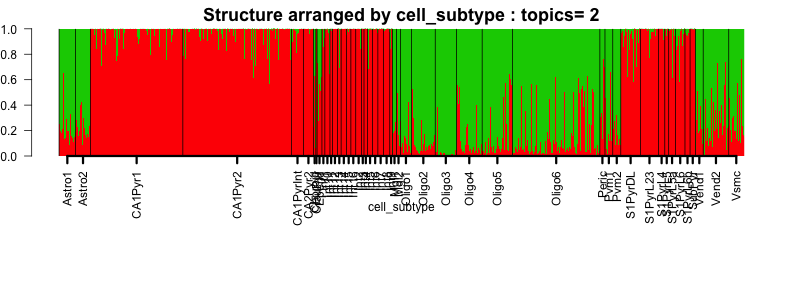
\includegraphics[height=2.5in]{../plots/Zeisel/clus_2/struct_clus_2_cell_subtype.png}
%        \raggedright 
%        \vspace{-0.5in} \qquad  \qquad  \caption{$k=2$}
%    \end{subfigure}    \\
%    \begin{subfigure}[t]{0.5\textwidth}
%        \raggedleft
%        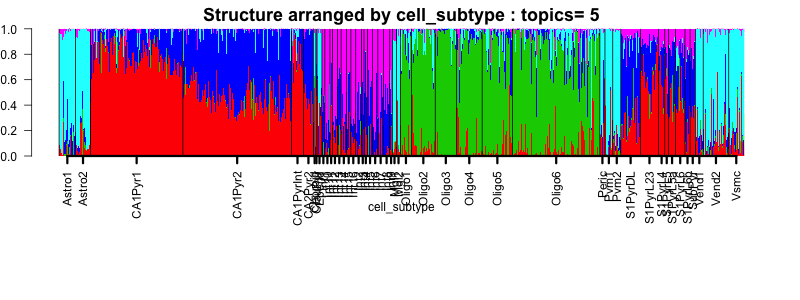
\includegraphics[height=2.5in]{../plots/Zeisel/clus_5/struct_clus_5_cell_subtype.png}
%        \raggedright
%        \vspace{-0.5in}  \qquad  \qquad \caption{$k=5$}
%    \end{subfigure}    \\
%    \begin{subfigure}[t]{0.5\textwidth}
%        \raggedleft
%        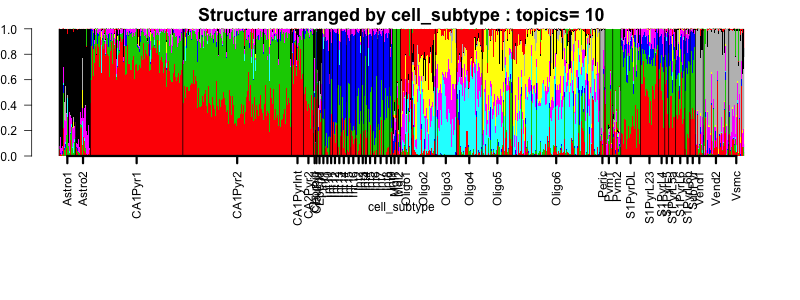
\includegraphics[height=2.5in]{../plots/Zeisel/clus_10/struct_clus_10_cell_subtype.png}
%        \raggedright
%        \vspace{-0.5in}  \qquad \qquad \caption{   $k=10$}
%    \end{subfigure}    
%    \caption{Structure plot of all  samples in Zeisel et al data \cite{Zeisel2015} arranged by the cell subtype labels that were determined by the authors using their BackSpin algorithm and subsequent marker gene annotations. Here we present the Structure plots for number of topics $k=2,5,10$. }
%    \end{figure*}


% \begin{figure*}[ht]
%    \raggedright
%     \begin{subfigure}[t]{1\textwidth}
%        \centering
%        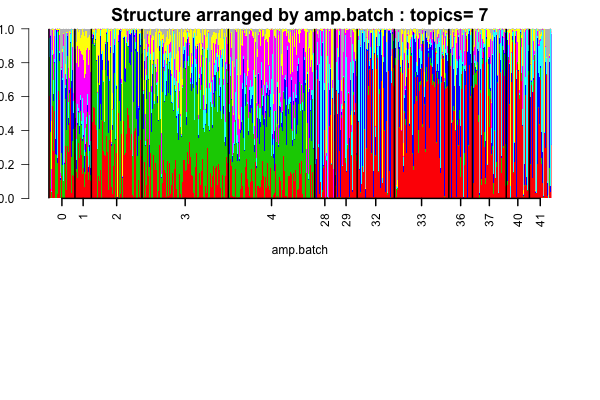
\includegraphics[height=2.5in, width=4.5in]{../plots/Jaitin_struct_clus_7_amp_batch.png}
%        \vspace{-1in} \qquad  \qquad  
%    \end{subfigure}    \\
%    \begin{subfigure}[t]{1\textwidth}
%       \centering
%        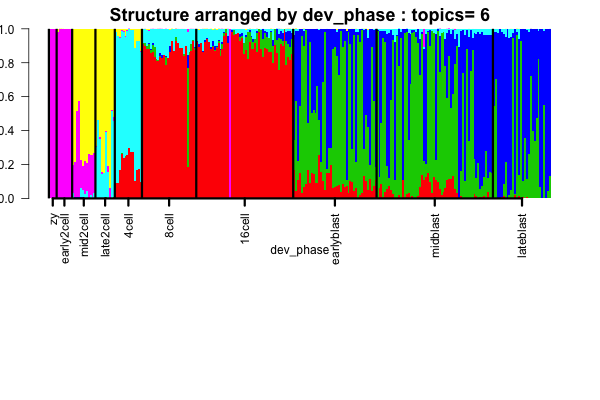
\includegraphics[height=2.5in, width=4.5in]{../plots/deng_structure_6.png}
%        \vspace{-0.5in}  \qquad \qquad 
%      \end{subfigure}
%    \caption{ (\textit{top panel})  Structure plot of the1041 single cells for K=7 of the Jaitin \textit{et al} data \cite{Jaitin2014} arranged by the amplification batch. It is observed that the clustering patterns within each batch are similar and so, either the amplification batch is driving the clustering or it is confounded with the actual biological effects, making it difficult to interpret these clusters. (\textit{bottom panel}) Structure plot of all samples for $K=6$ of Deng et al data \cite{Deng2014}, arranged by the preimplantation development phases of the cells and within each phase, arranged in the same order as in the data. Some developmental phases are represented by a single cluster, for example- \textit{zygote/early2cell} while some developmental phases can be written as a mix of two clusters or more clusters.}. 
% \label{fig:fig3}
% \end{figure*}
% 

\begin{figure*}[ht]
\centering
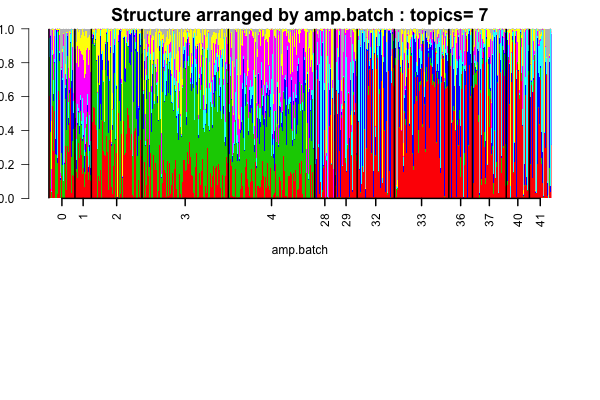
\includegraphics[height=2.5in, width=4.5in]{../plots/Jaitin_struct_clus_7_amp_batch.png}
\caption{Structure plot of estimated cluster membership proportions for $K=7$ clusters fit to 1041 single cells from \cite{Jaitin2014}. The samples are ordered so that samples from the same amplification batch are adjacent. In this analysis the samples do not appear to form clearly-defined clusters, with each sample being allocated membership in several ``clusters". Visually, samples from the same amplification batch tend to be assigned similar membership proportions, suggesting that batch effects are likely contributing to the inferred clustering.}
\label{fig:fig3}
\end{figure*}



\begin{figure*}[ht]
\centering
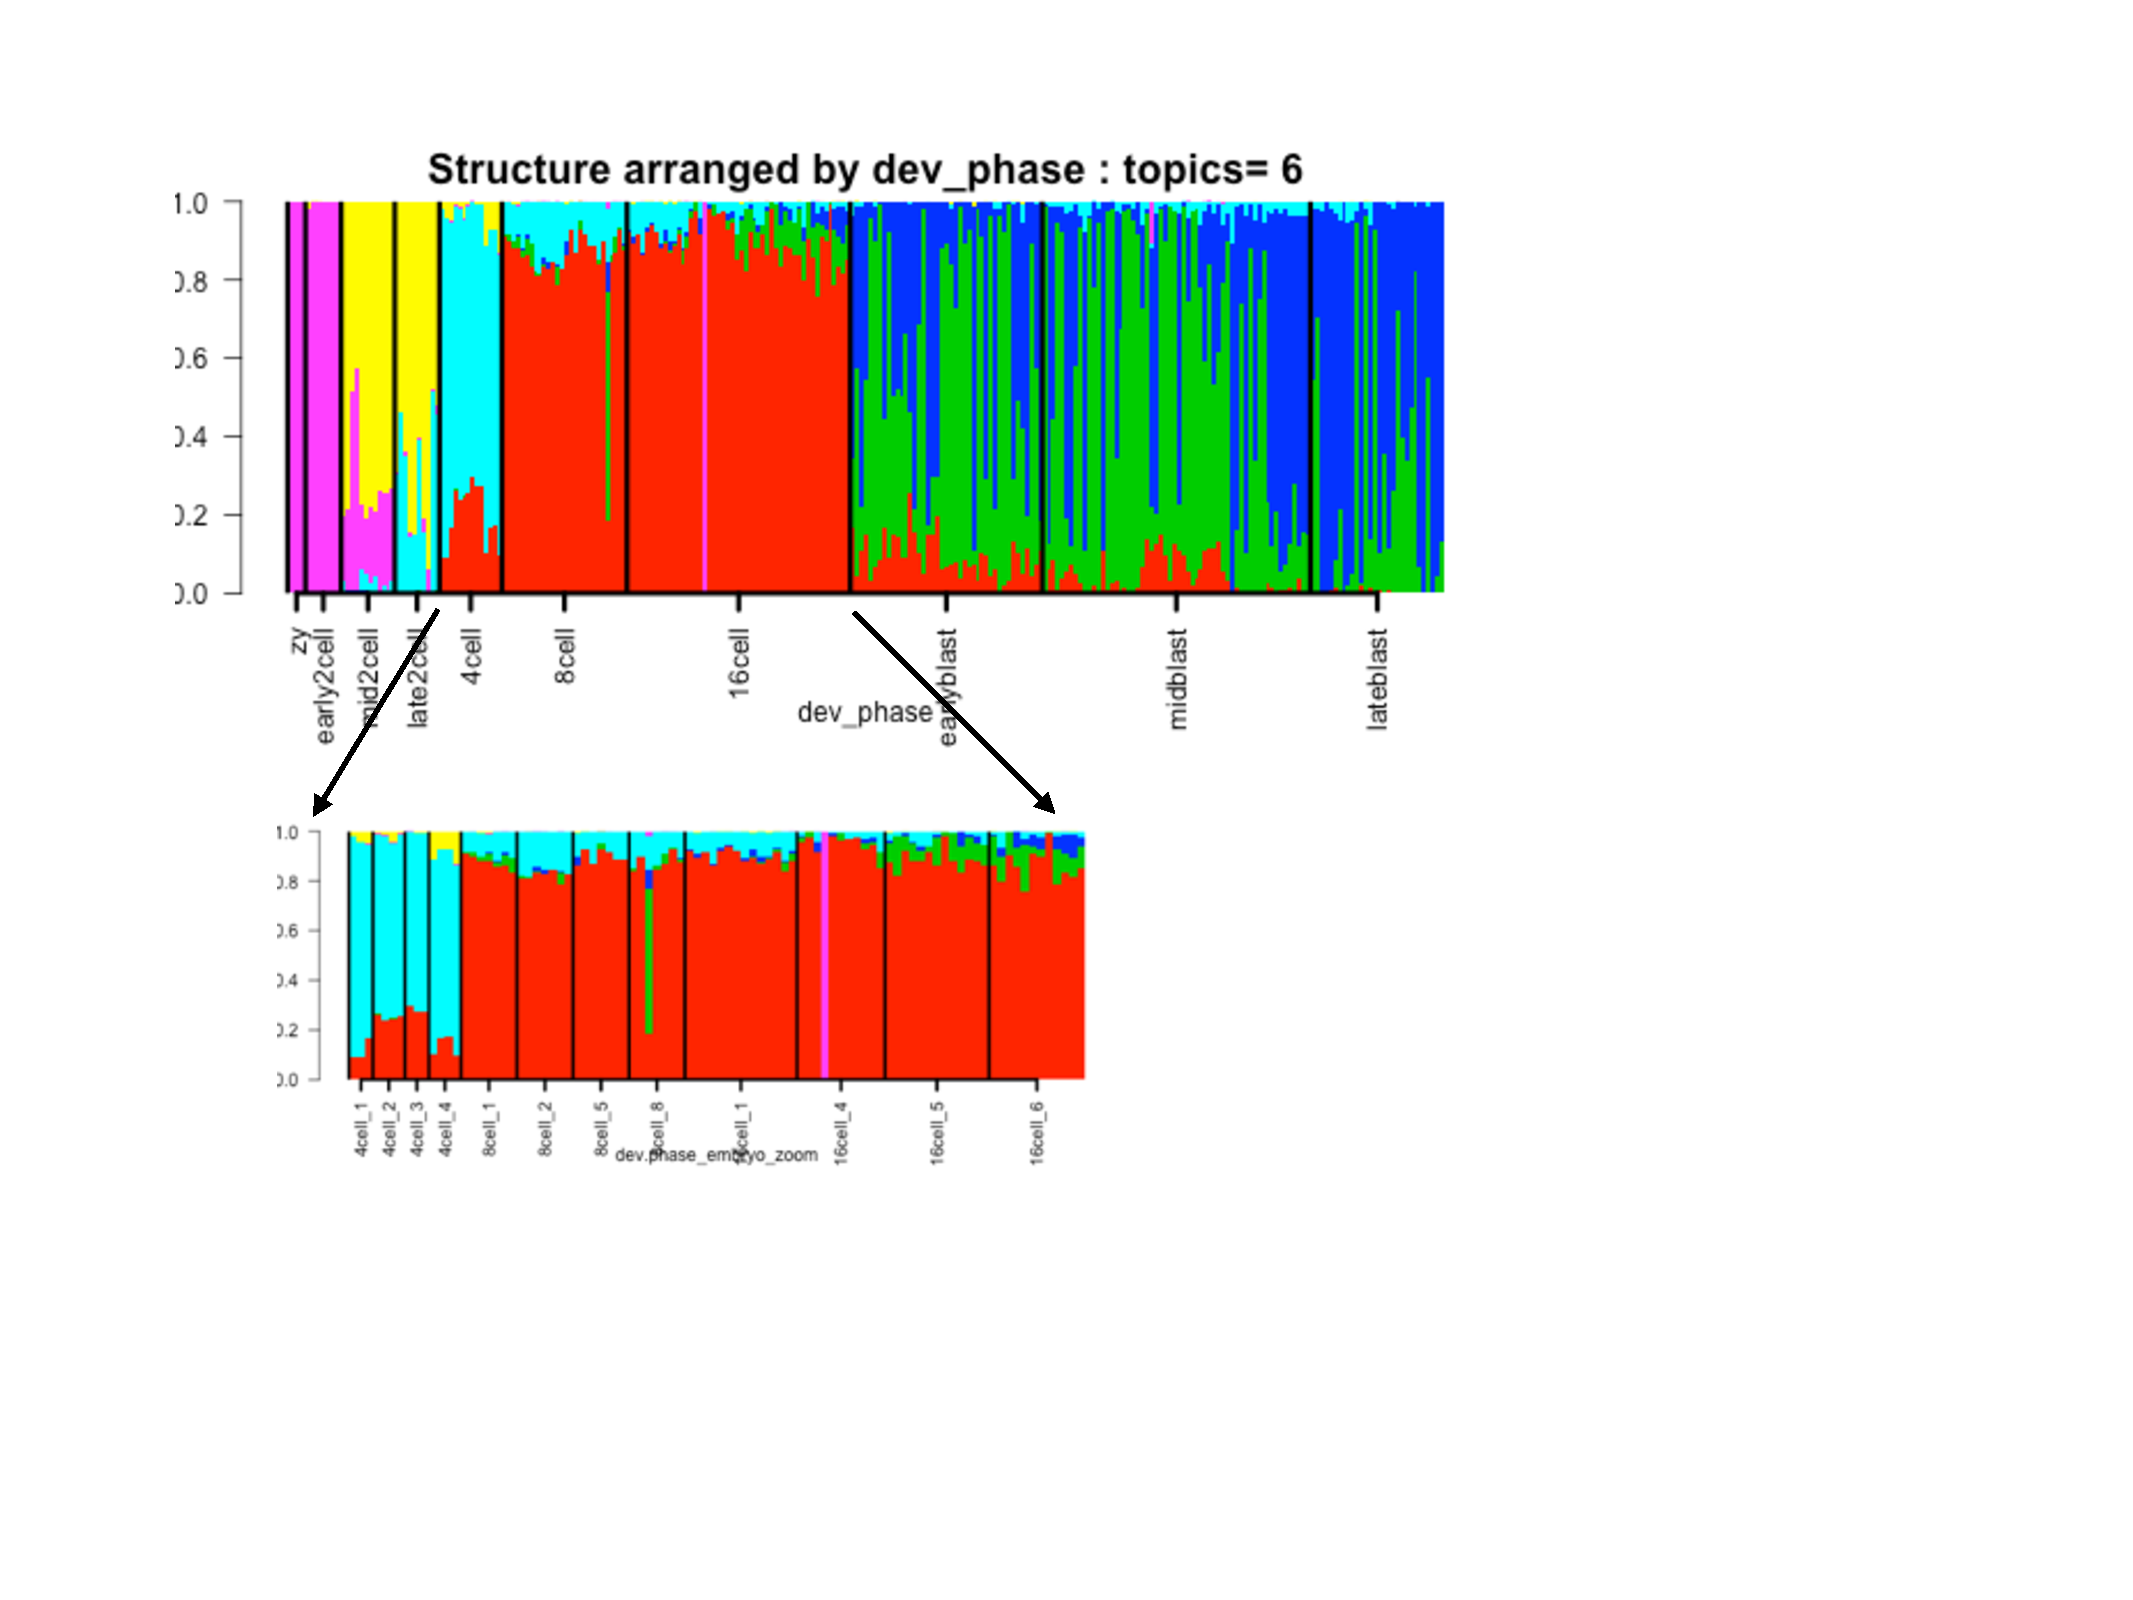
\includegraphics[height=4in, width=5.5in]{../plots/deng_structure_6.pdf}
\caption{Structure plot of estimated cluster membership proportions for $K=6$ clusters fit to xxx single cells from  \cite{Deng2014}. The cells are ordered
by their preimplantation development phase (and within each phase, arranged in the same order as in the data file). While the very earliest developmental phases 
(\textit{zygote/early2cell}) are essentially assigned to a single cluster, others are represented as a mix of two or more clusters. This illustrates the idea that
structure of single-cell data may in some cases be better captured by a mixed membership model than by simple discrete clusters.}
\label{fig:fig4}
\end{figure*}


 \clearpage
 
 \subsection{Supplemental figures}
 
  \begin{figure*}[ht]
    \centering    
     \begin{subfigure}[t]{0.5\textwidth}
        \centering
        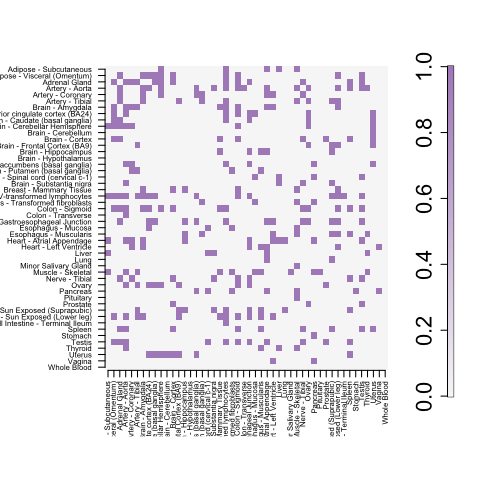
\includegraphics[height=2.5in]{../plots/hierarchy_F_thin_0_01.png}
        \caption{hierarchy thin 0.01}
    \end{subfigure}%
    ~
    \begin{subfigure}[t]{0.5\textwidth}
        \centering
        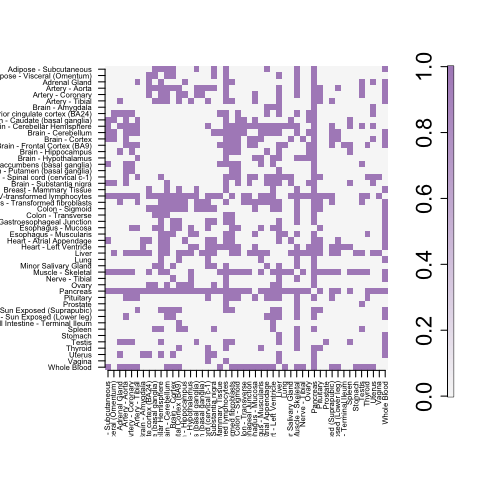
\includegraphics[height=2.5in]{../plots/admixture_F_thin_0_01.png}
        \caption{admixture thin 0.01}
    \end{subfigure}\\
    
     \begin{subfigure}[t]{0.5\textwidth}
        \centering
        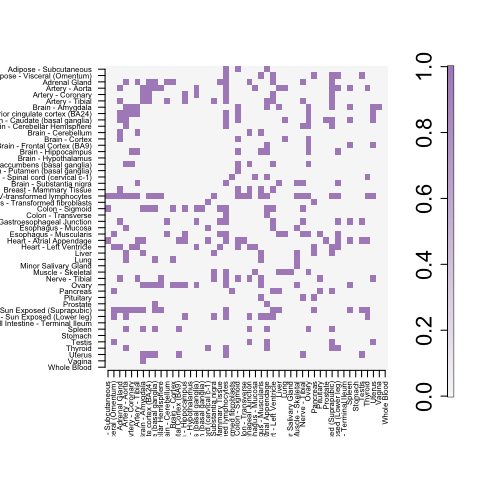
\includegraphics[height=2.5in]{../plots/hierarchy_F_thin_0_001.png}
        \caption{hierarchy 0.001}
    \end{subfigure}%
    ~
    \begin{subfigure}[t]{0.5\textwidth}
        \centering
        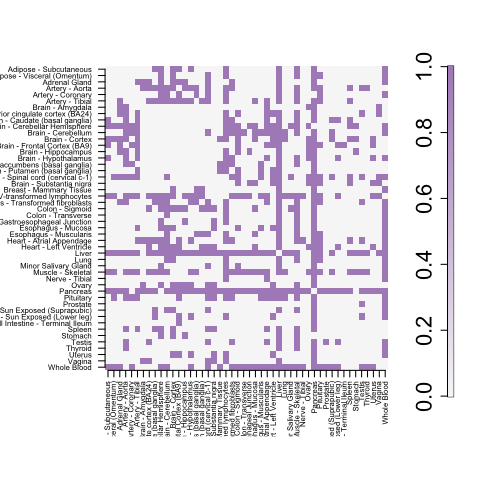
\includegraphics[height=2.5in]{../plots/admixture_F_thin_0_001.png}
        \caption{admixture thin 0.001}
    \end{subfigure}\\

 \caption{A comparison of ``accuracy" of hierarchical vs model-based clustering on thinned GTEX data, with thinning parameter $p_{thin}=0.001$ and $p_{thin}=0.0001$.  For each pair of tissues from the GTEX data we assessed whether or not each clustering method (with $K=2$ clusters) separated the samples according to their actual tissue of origin, with successful separation indicated by a filled square. As expected, thinning deteriorate accuracy compared with the unthinned data (Figure \ref{fig:fig3}), but the model-based method remains more successful than the hierarchical clustering in separating the samples by tissue or origin.}
 \label{fig:figS2}
\end{figure*}


